\section*{Methodology}
The research methodology is summarized by the diagram given in Figure \ref{methodology-new}. 

\begin{figure}
\centering
%\begin{center}
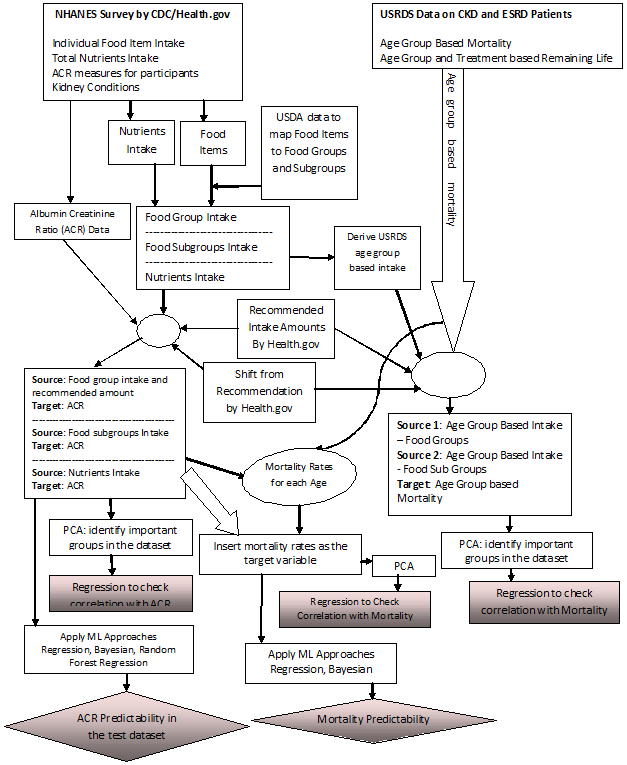
\includegraphics[scale=0.48]{./images/methodologies-enhanced}
%\end{center}
\caption{\textbf{Methodology in a Diagram}}
\label{methodology-new}
\end{figure}

\subsection*{Methodology Overview}
 Dietary survey dataset from NHANES, and age group based CKD Mortality dataset from USRDS, Food Grouping and subgrouping datasets from USDA, Shift Recommendation study by CDC are utilized in this study. NHANES survey dataset by CDC/Health.gov have data with the dietary habits and ACR values for close to 10,000 individuals.  This study utilized Principal Component Analysis to identify the most important food groups and subgroups affecting the ACR value and the CKD Mortality rates.  Statistical regression and factor analysis were then applied to understand the correlation between ACR, and Mortality rates to dietary patterns. We identified important food groups and subgroups that affect ACR and Mortality positively or negatively. The findings were then compared against the Dietray Recommendations shift  \cite{Health2015} by CDC to compare how the recommendations shift affect CKD patients.

\subsection*{Study Selection}
For dietary patterns, CKD measures (such as Albumin to Creatinine Ratio - ACR), and Kidney condition measures, a dataset from the National Health and Nutrition Examination Survey on dietary habits conducted by the CDC \cite{CDC2015} was used. The survey has data from 1996 to 2016 \cite{CDC2015}. This study primarily utilized data for 2015-2016. The survey recorded 24 hours individual food item intake amount. Two surveys were taken within 3 to 10 days apart. Each survey provided food item intake amounts in a day and recorded the diet style as well as diet-restrictions. Individual food items are represented using USDA food code. The survey also provided total nutrients data. CDC also released examination, laboratory, demographics, and other related data for those participants. This study explored and utilized examination data such as Kidney Condition data, laboratory data such as ACR data \& Blood Pressure data, and demographics data for age.
 
For mortality and survival information, dataset from the United States Renal Data System (USRDS) on CKD and ESRD \cite{USRDS2015} \cite{USRDS2018} were utilized. “USRDS investigates the transition of care from CKD to ESRD and end-of-life care for those with advanced kidney disease” \cite{USRDSAnnual2018}. USRDS also releases data on the Incidence, Prevalence, Patient Characteristics, and Treatment Modalities on CKD, and ESRD patients. USRDS  reports survival and mortality using metrics such as Mortality rates, Total Mortality Count,  90 day survival for dialysis and/or transplantation patients,  10 year survival for dialysis and/or transplantation patients, Average Expected remaining lifetime with or without pre-condition and treatment options used.  The data are either aggregated or patient specific detail data. This research utilized only the public dataset i.e. age-group based aggregated data. In couple of experiments, aggregated age-group based data from USRDS was mapped to specific age for NHANES data for each age and participants.

The dietary survey data (NHANES) represented the food items taken by the participants using USDA food codes \cite{ARS2016} \cite{CDC2004} \cite{USDA2010}. Hence, USDA food codes \cite{ARS2016} \cite{CDC2004} \cite{USDA2010} are used to assign food groups and subgroups to the NHANES \cite{CDC2015} survey data to properly group/subgroup the dietary intake of the participants with some customizations.

The shift recommendation study \cite{Health2015}  as part of national act studied the current food habits of U.S. population and identified compliance to provide guidance based on current scientific and medical knowledge. Based on their study, they have recommended areas where adjustments wil be important to the dietary recommendations so that it becomes easier for the people to adhere to the recommendations.  The dietary guidelines provided guidelines that encourage `healthy eating patterns, recognize that individuals will need to make shifts in their food and beverage choices to achieve a healthy pattern, and acknowledge that all segments of our society have a role to play in supporting healthy choices''. These Guidelines also embody the idea that a healthy eating pattern is an adaptable framework in which individuals can enjoy foods that meet their personal, cultural, and traditional preferences while being within their budget. CDC also provided suggestions on how to change the dietary habits. \cite{Health2015}.

\subsection*{Data Synthesis}
NHANES survey data as provided for two days are averaged to get the intake amount for one day. Both individual food item data and nutrients intake data are averaged. USDA food codes are used to map food items to food groups and subgroups. The same food grouping and subgrouping approach utilizing USDA as used by the shift recommendation study is used with negligible exceptions.

ACR and Kidney condition data for each individual are merged with the averaged food groups, subgroups, and nutrients data for the non-age group based studies. This data was further complemented with the food group recommendations data from health.gov, and mortality rate by age from the USRDS. ACR values and mortality rate  are used as the target variables.

In another mortality experiment, the above synthesized datasets were aggregated for USRDS age  groups to calculate average food group/subgroup intake by age groups. 

PCA was applied to find out important food groups and subgroups while regression was applied to find potential associations with ACR and Mortality. 